%--------------------------------------------------
\section{Effect of the small size of W+jets MC sample on its shape}
A limited amount of W$jj$ Monte Carlo (less than $2x$ the data) is a
major source of systematic uncertainty. In order to estimate the
associated error we use the $m_{jj}$ shape from the MC to generate
$1000$ toy datasets and repeat the fit using each one of them as a
template. Note that the event counts in each bin are allowed to
fluctuate independently along a Gaussian with mean and error given by
the original dataset. A comparison between the results using the
original template and the $1K$ fits using the Toy MC are provided in
Table~\ref{table:WjjMCSystResults}, while fits to the extracted yields
are displayed in Figure~\ref{fig:WjjMCSystFit}. Since the uncertainty
on the yields is a combination of systematics as well as statistics we
extract the error associated with limited Monte Carlo via
$\sigma^2_{Tot}=\sigma^2_{stat}+\sigma^2_{MCsyst}$.

%%The resultant uncertainty is 121 events, with it's impact 
%%on the fit shown in Figure~\ref{fig:WjjMCSystError}.
%%%%%%%
\begin{table}[tb]
\caption{Results of the fits using 1000 Toy MC W$jj$ templates.}
\begin{center}
\begin{tabular}{|c|c|c|c|}
\hline
   Quantity
 & Expected
 & Fitted Mean
 & Fitted $\sigma$ \cr
\hline
\vspace{-0.5cm} & & \cr
{WW-Yield}    &  1014 &  1027 $\pm$ 6 & 185 $\pm$ 5 \cr
\hline
{W$jj$-Yield} & 33143 & 33129 $\pm$ 6 & 193 $\pm$ 5 \cr
\hline
\end{tabular}
\end{center}
\label{table:WjjMCSystResults}
\end{table}

In addition, we plan to use W+jets templates from several different Monte Carlo 
generators (\textit{e.g.,} \textit{MadGraph}, \textit{Sherpa}, 
\textit{MCFM}) to assess the overall systematics from the 
imperfect understanding of the W+jets spectrum.
We also plan to attempt other cross checks by using data-driven techniques 
(\textit{e.g.}, by constraining the template in the sidebands 
or by using a $m_{jj}$ template from Z+jets events, which have 
similar kinematics).
%%%%%%%%%%%%%%%%%%%%%%%%%%%%
%%%%%%%
\begin{figure}[h!] {\centering
\unitlength=0.33\linewidth
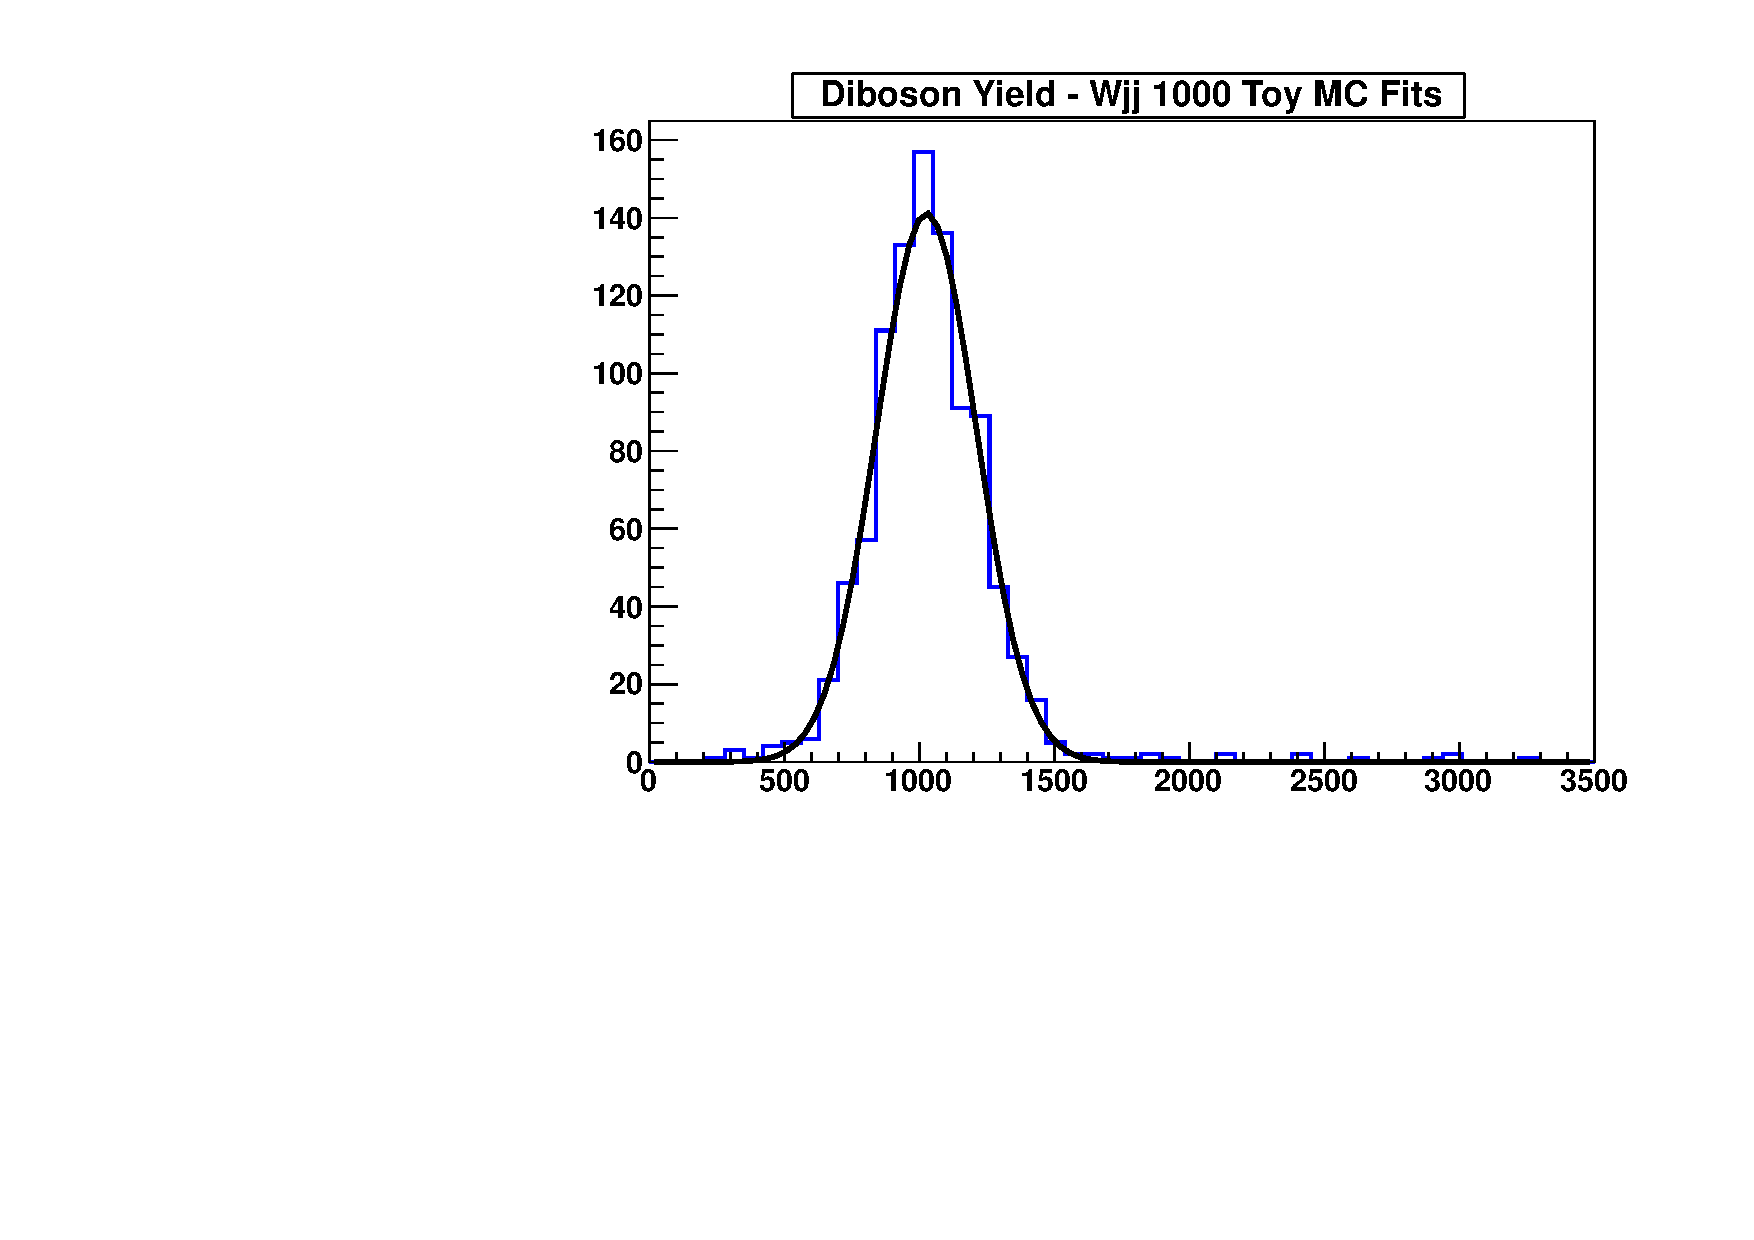
\includegraphics[width=0.48\textwidth]{figs/ToyMCWjjTemplateFit_WWYield.pdf}
\put(-0.80,0.0){(a)} 
\unitlength=0.33\linewidth
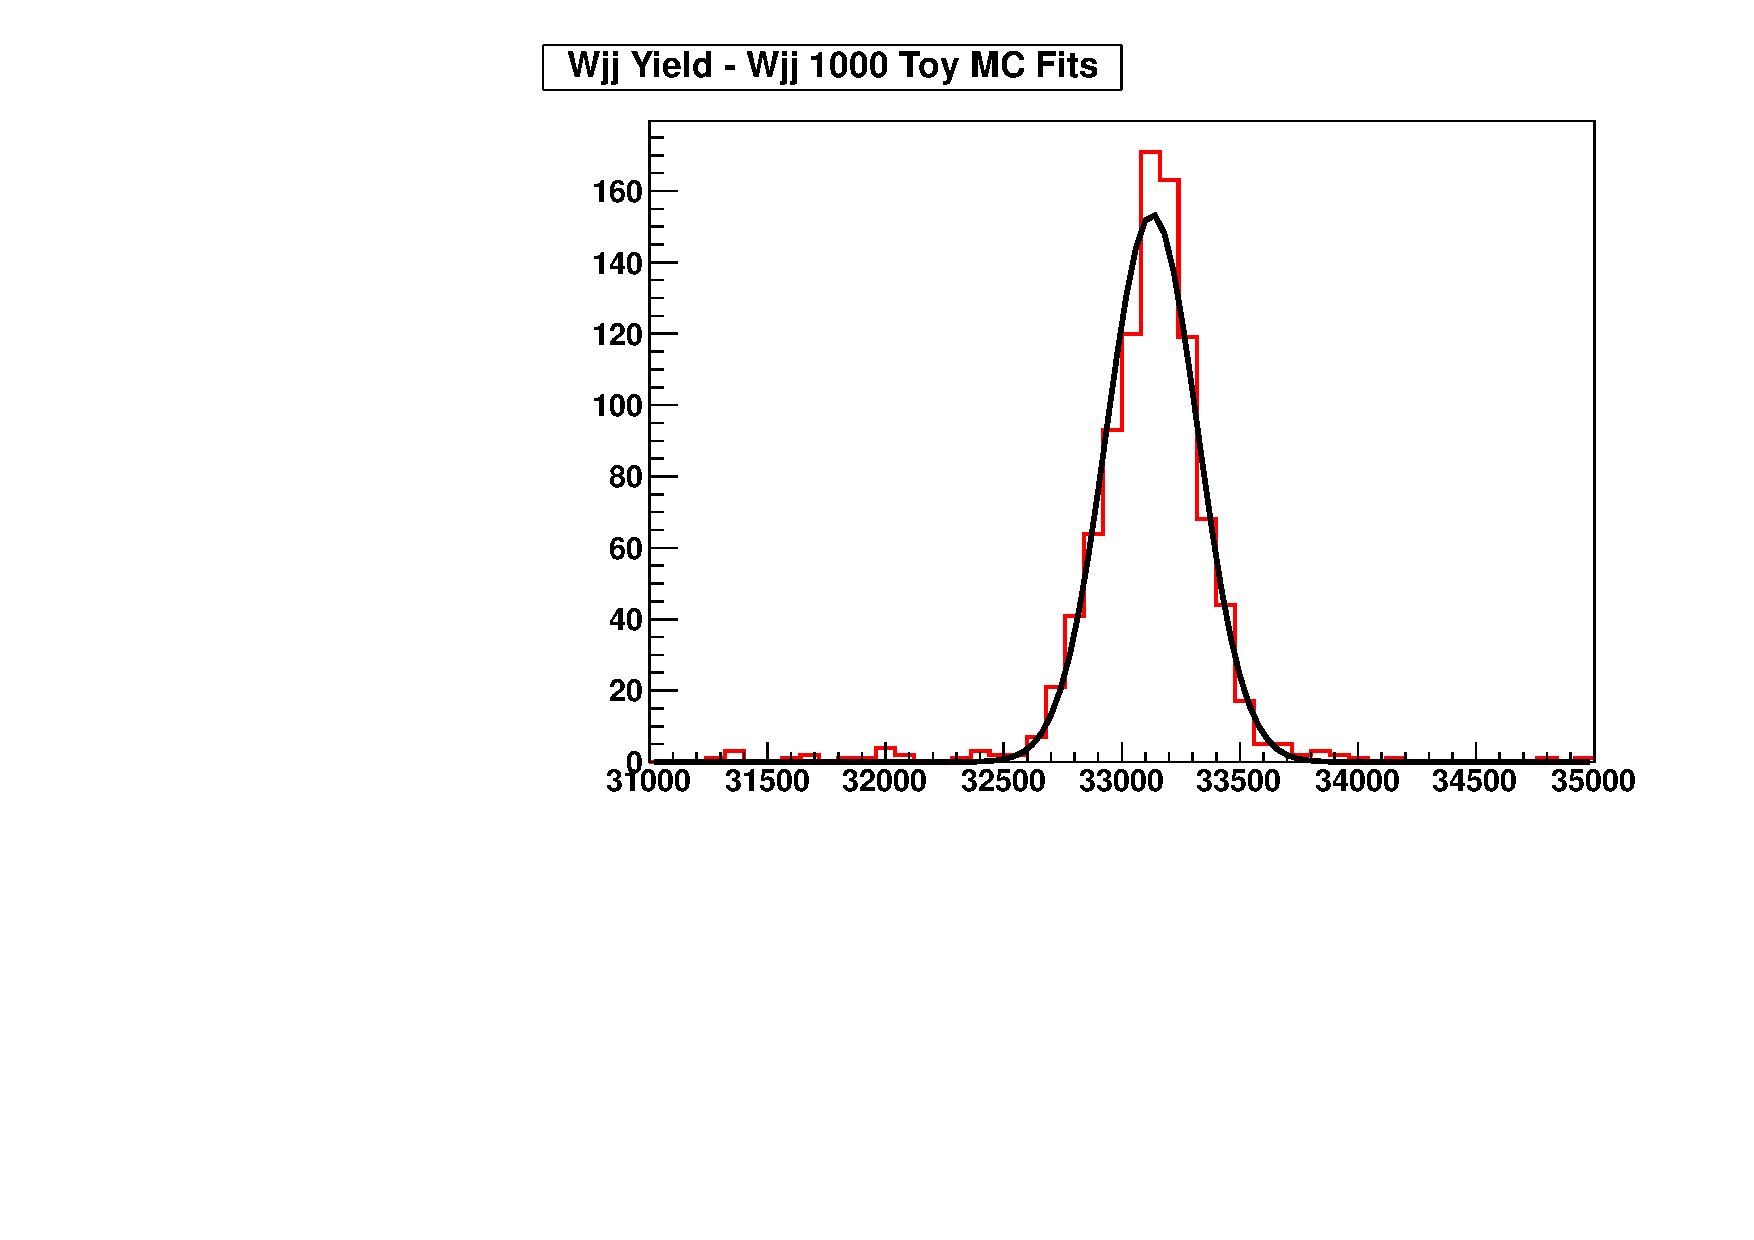
\includegraphics[width=0.48\textwidth]{figs/ToyMCWjjTemplateFit_WjjYield.pdf}
\put(-0.80,0.0){(b)} 
\caption{(a) WW and (b) W$jj$ Yields obtained from the 1000 fits using Toy MC W$jj$ templates.} 
\label{fig:WjjMCSystFit}}
\end{figure}
%%%%%%%
%%%%%%%
%\begin{figure}[h!] {\centering
%\unitlength=0.33\linewidth
%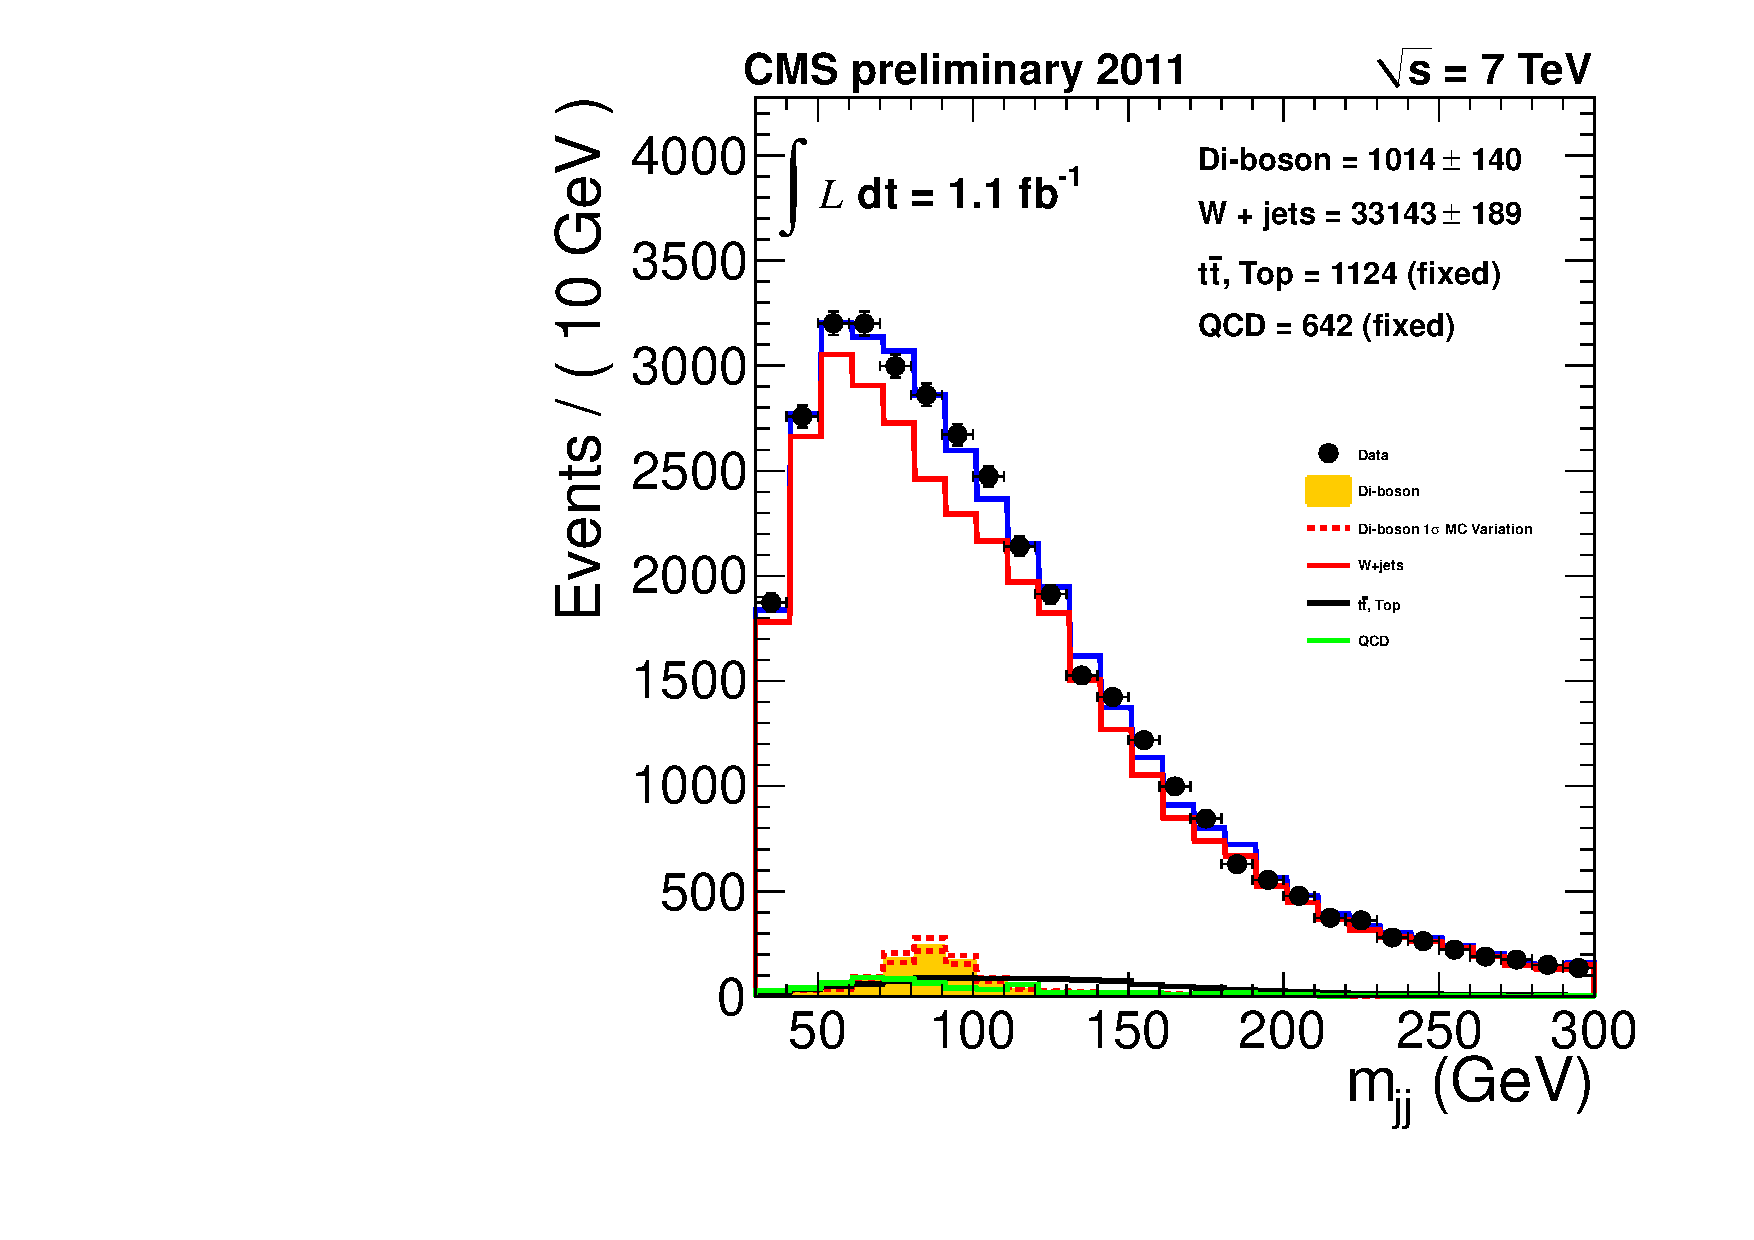
\includegraphics[width=0.48\textwidth]{figs/WjjMCSyst_mJJ-combined-fit.pdf}
%\put(-0.80,0.0){(a)} 
%\unitlength=0.33\linewidth
%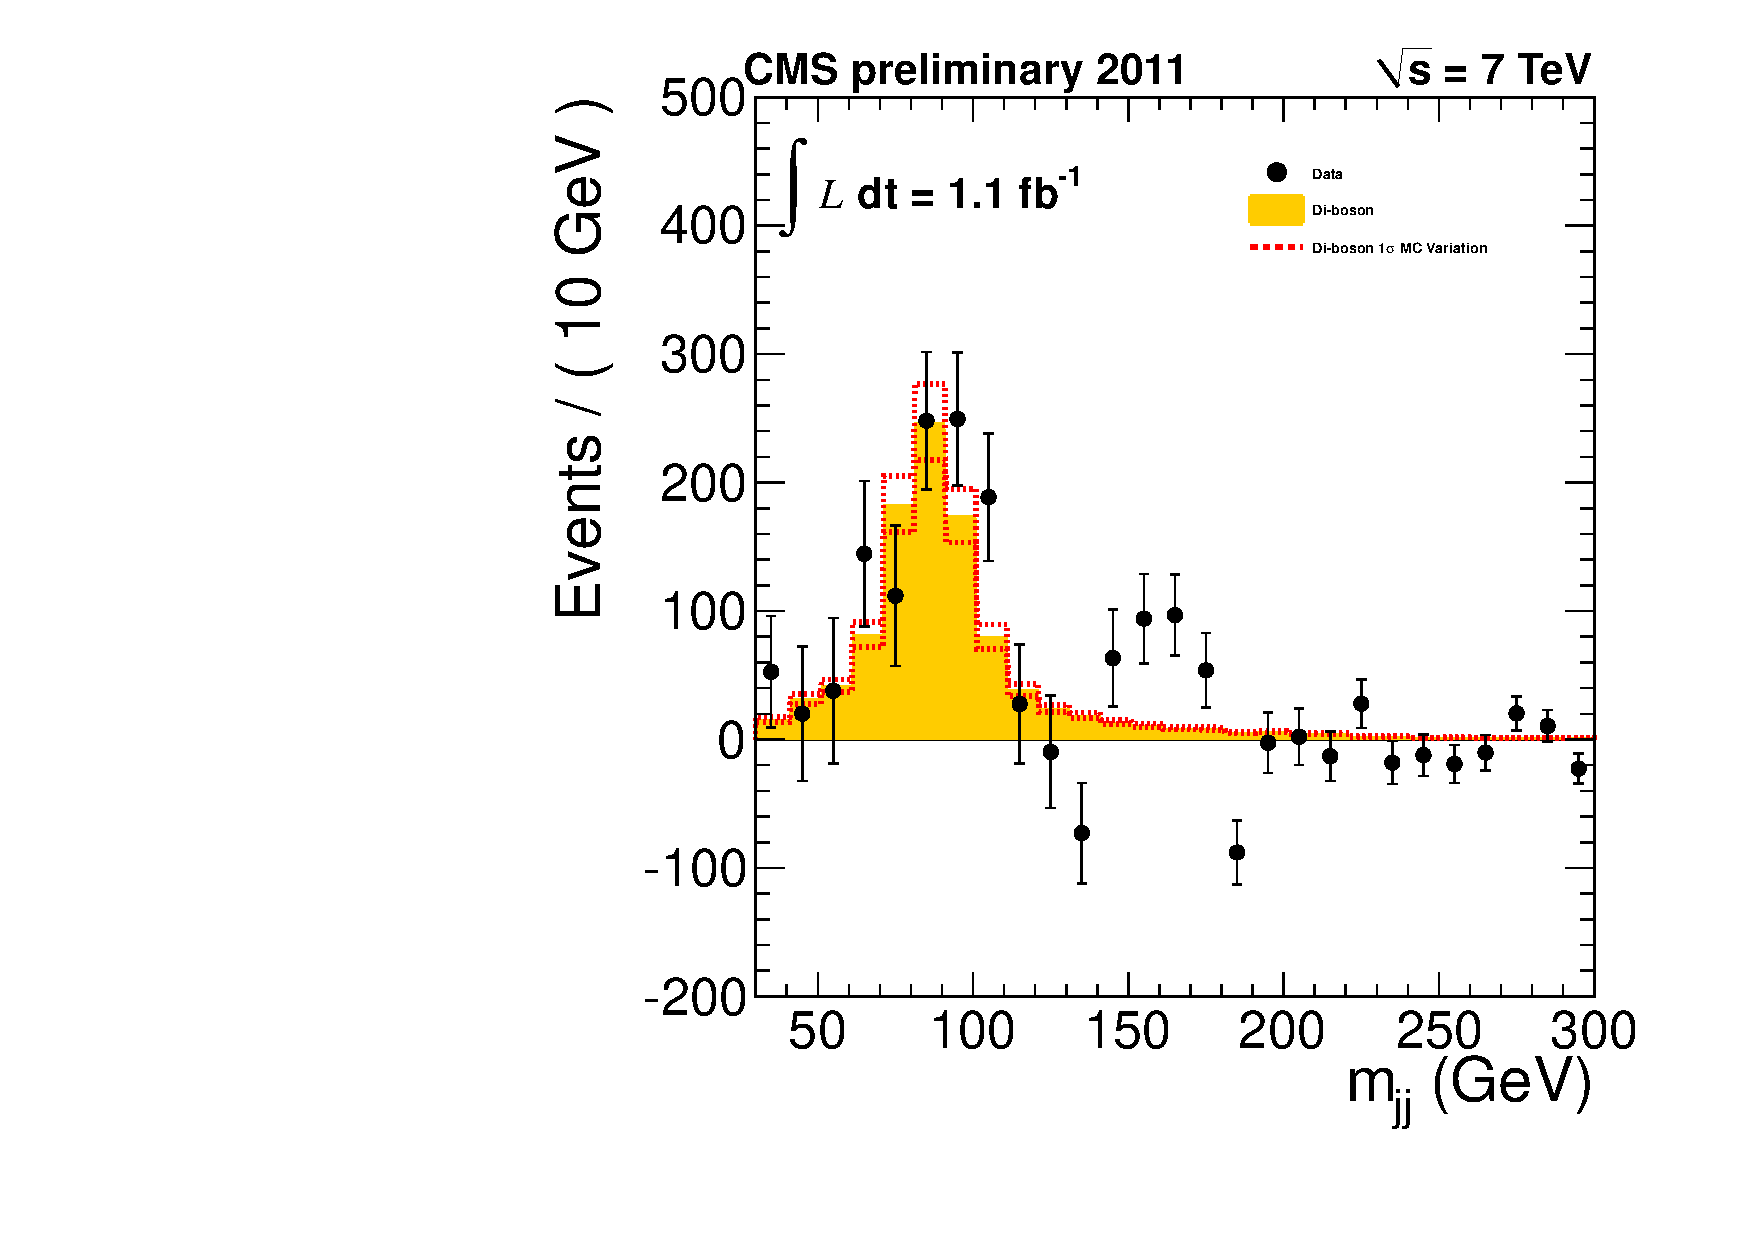
\includegraphics[width=0.48\textwidth]{figs/WjjMCSyst_mJJ-combined-fit-subtracted.pdf}
%\put(-0.80,0.0){(b)} 
%\caption{Impact of the error due to limited W$jj$ (dotted line) before (a) and after (b) the subtraction of the background components.} 
%\label{fig:WjjMCSystError}}}
%\end{figure}
%%%%%%%%
%%%%%%%%%%%%%%%%%%%%%%%%%%%%
